\chapter{Rappresentazione della scacchiera e dei pezzi} %\label{1cap:spinta_laterale}
% [titolo ridotto se non ci dovesse stare] {titolo completo}
%

\begin{citazione}
    In questo capitolo viene mostrato passo passo un procedimento guida alla realizzazione di un motore scacchistico
\end{citazione}

\newpage

\section{Introduzione} %\label{1sec:scopo}
Il primo passo dello sviluppo di un motore scacchistico è decidere come si vuole rappresentare
la scacchiera , si tratta di una scelta fondamentale,non solo perché in seguito ci permetterà
di testare le funzioni che andremo a implementare, ma anche perché è nella scacchiera che ,generalmente,
viene conservato lo stato generale della partita.\footnote{per stato di una partita si intendono informazioni come
    informazioni su chi ha diritto di muovere, i permessi di arrocco,lo stato della regola delle 50 mosse etc}
Inoltre il tipo di codifica può influenzare la rapidità
e la facilità col quale possiamo accedere alle informazioni sullo stato corrente dei pezzi
e come vedremo in seguito è in grado di influenzare funzioni come la generazione delle mosse.
Non è raro per motori scacchistici particolarmente complessi l'utilizzo di più tipi di board in base
al tipo di informazione da conservare e all'utilizzo che se ne vuole fare.
Per la rappresentazione di una scacchiera sono chiaramente possibili moltissime scelte, di seguito
verranno illustrate alcune tra le più popolari ed utilizzate.

\section{Rappresentazione della scacchiera Pezzocentrica}
Si definisce rappresentazione pezzocentrica, un qualsiasi tipo di rappresentazione della scacchiera che mantiene liste
array o set dei pezzi attualmente presenti sulla scacchiera con annesse le informazioni sulle caselle da essi occupate.
Le rappresentazioni più comuni sono:
\subsubsection{Piece-Lists}
liste o array di ogni pezzo sulla scacchiera,ogni elemento della lista o dell'array associa un pezzo
alla casella che esso occupa .le caratteristiche di ogni pezzo (colore,tipo etc)
possono essere associate all'indice dell'array in cui si trovano o essere presenti in ulteriori array
o liste esterne. \emph{un'implementazione pratica di una Piece-List verrà mostrata in seguito all'interno
    di questo capitolo}

\subsubsection{Bitboards}
Una Bitboard è una struttura dati specifica per i giochi da tavolo,
si tratta in sostanza  di una struttura dati in grado di immagazzinare lo stato di ogni casella della
scacchiera all'interno di una parola \footnote{Una parola è un gruppo di bit di una determinata dimensione che sono gestiti come unità dal set di istruzioni o dall'hardware di un processore} di 64 bit.
Vediamo un esempio pratico, immaginiamo di avere una scacchiera che si trova nello stato di default di inizio
partita:
\begin{figure}
    \centering
    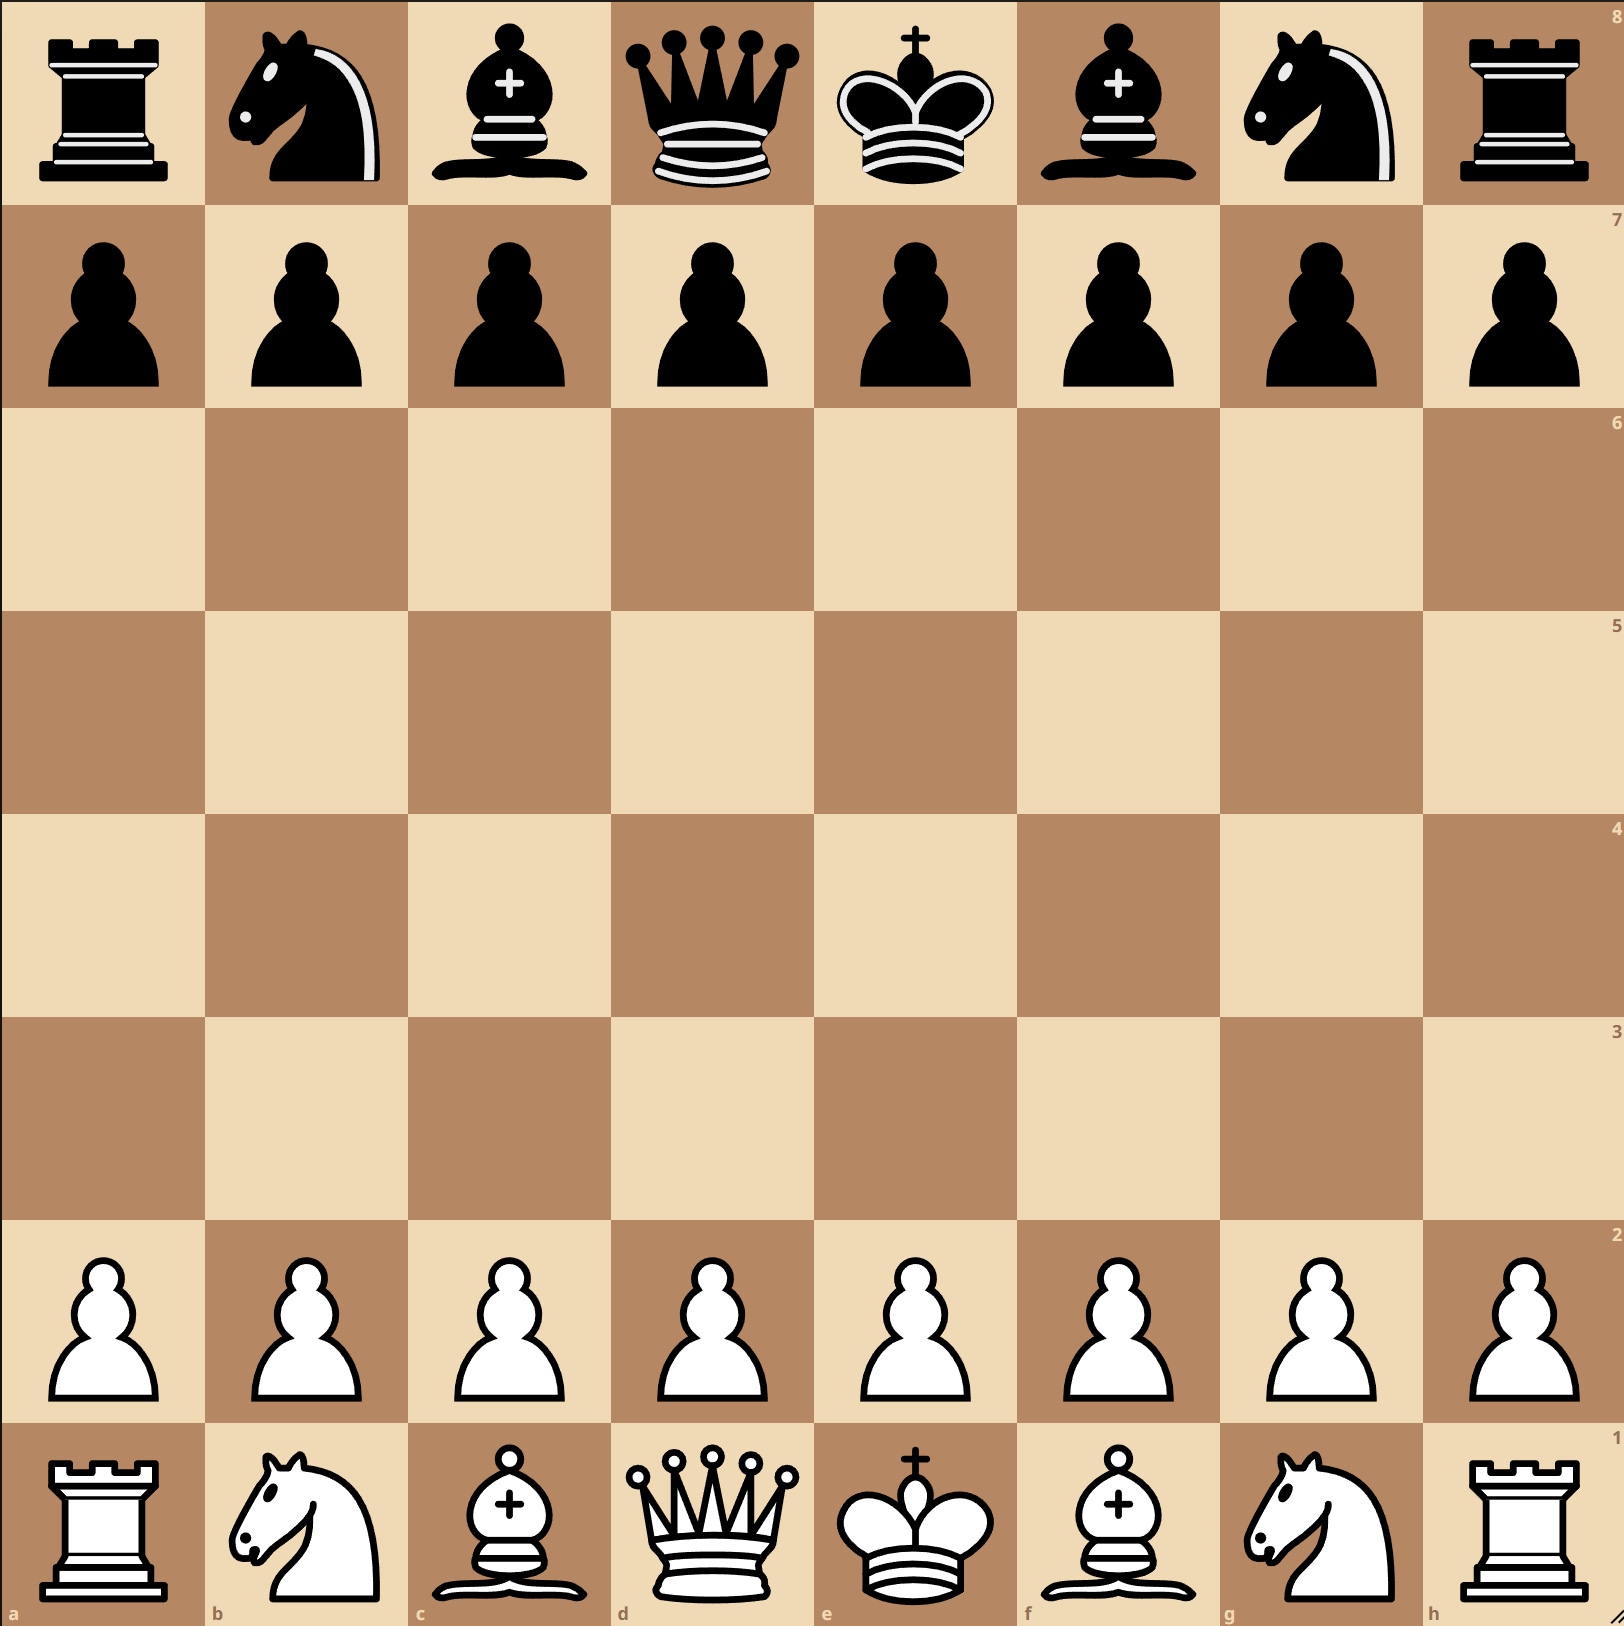
\includegraphics[width=\linewidth/2] {scacchiera.png}
    \caption{Scacchiera nella classica posizione di finale con alfieri di colore opposto }
\end{figure}

Una bitboard tipica è quella che ci permette di sapere in quali caselle è presente un pedone
nero,per costruirla, operando casella per casella, ci poniamo una domanda "in questa casella
è presente un pedone nero?" se si allora quella casella viene marcata con un 1 , altrimenti viene
marcata con uno 0, il risultato di questa traduzione diventa in questo caso:
\begin{figure}
    \centering
    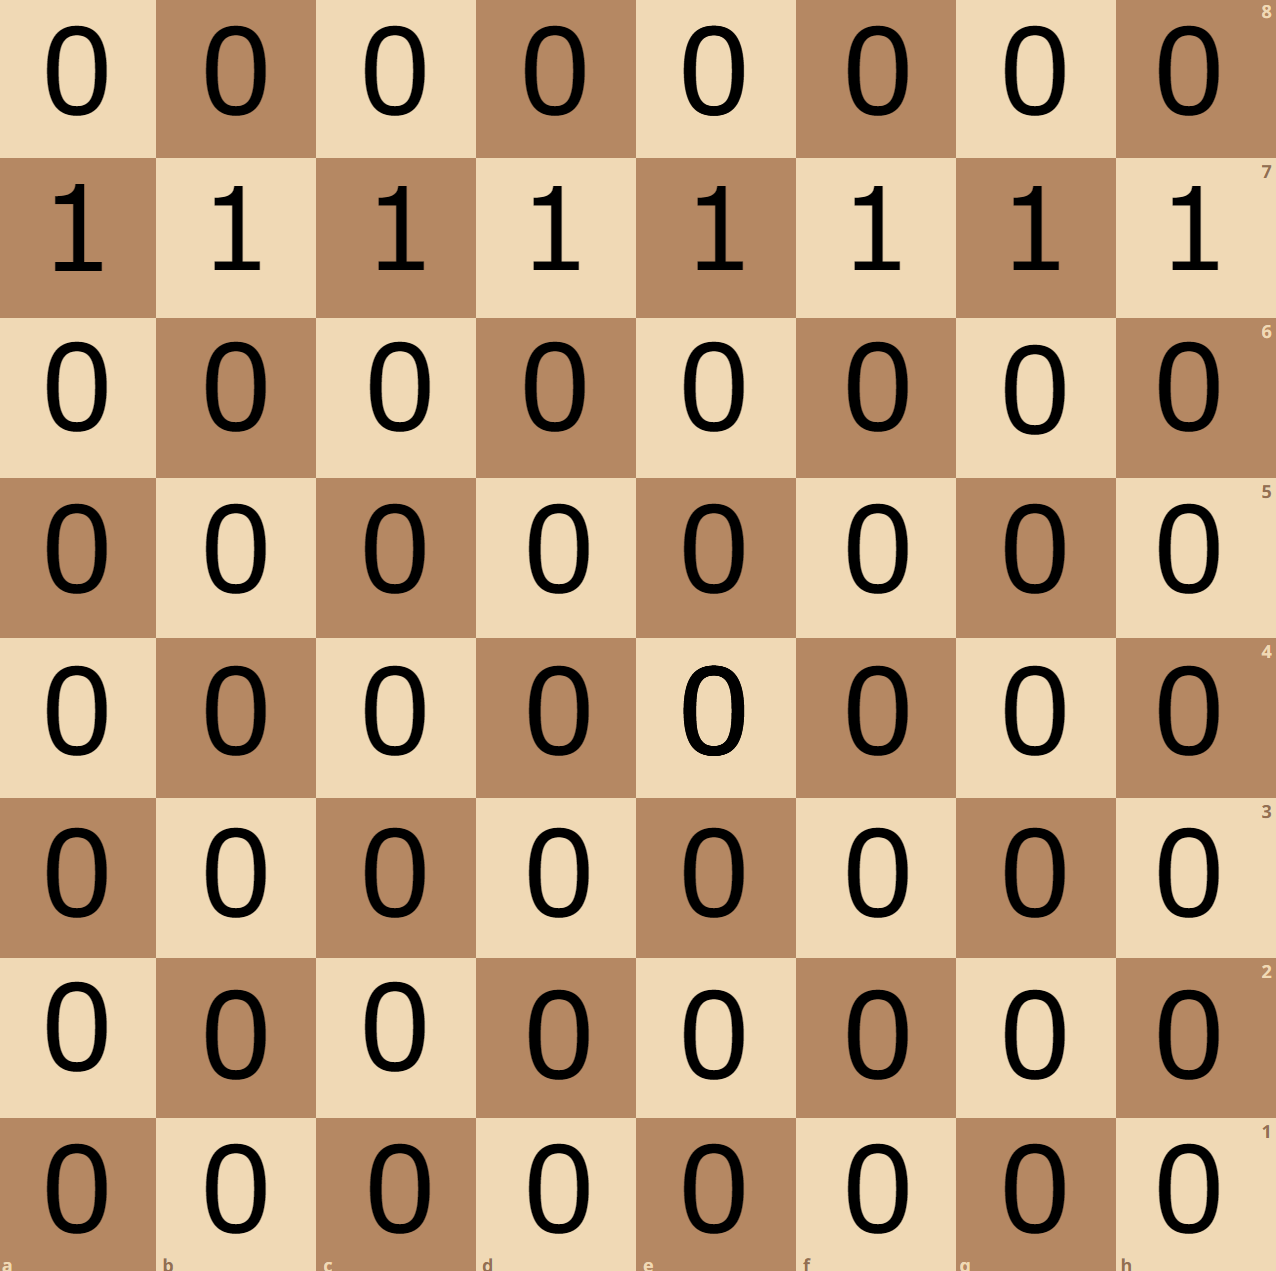
\includegraphics[width=\linewidth/2] {bitboard.png}
    \caption{bitboard}
\end{figure}
La bitboard che codifica questa informazione sarà quindi la parola di 64 bit 00000000 11111111 00000000 00000000 00000000
00000000 00000000 00000000
\subsubsection{Piece-Sets}
rappresentazione con set con un bit per ogni pezzo dentro una parola a 32 bit o 2 parole a 16 bit per ogni lato.
i Piece-sets hanno  delle somiglianze con le bitboards, ma ogni  bit del set non è   direttamente correlato ad una casella,
ma ad un indice  dentro ad una  piece-list. Spesso la bit-position di un  piece-set  implica
, di che tipo e colore il pezzo è. - mentre le  bitboards solitamente mantengono set distinti
per pezzi diversi.

\begin{figure}
    \centering
    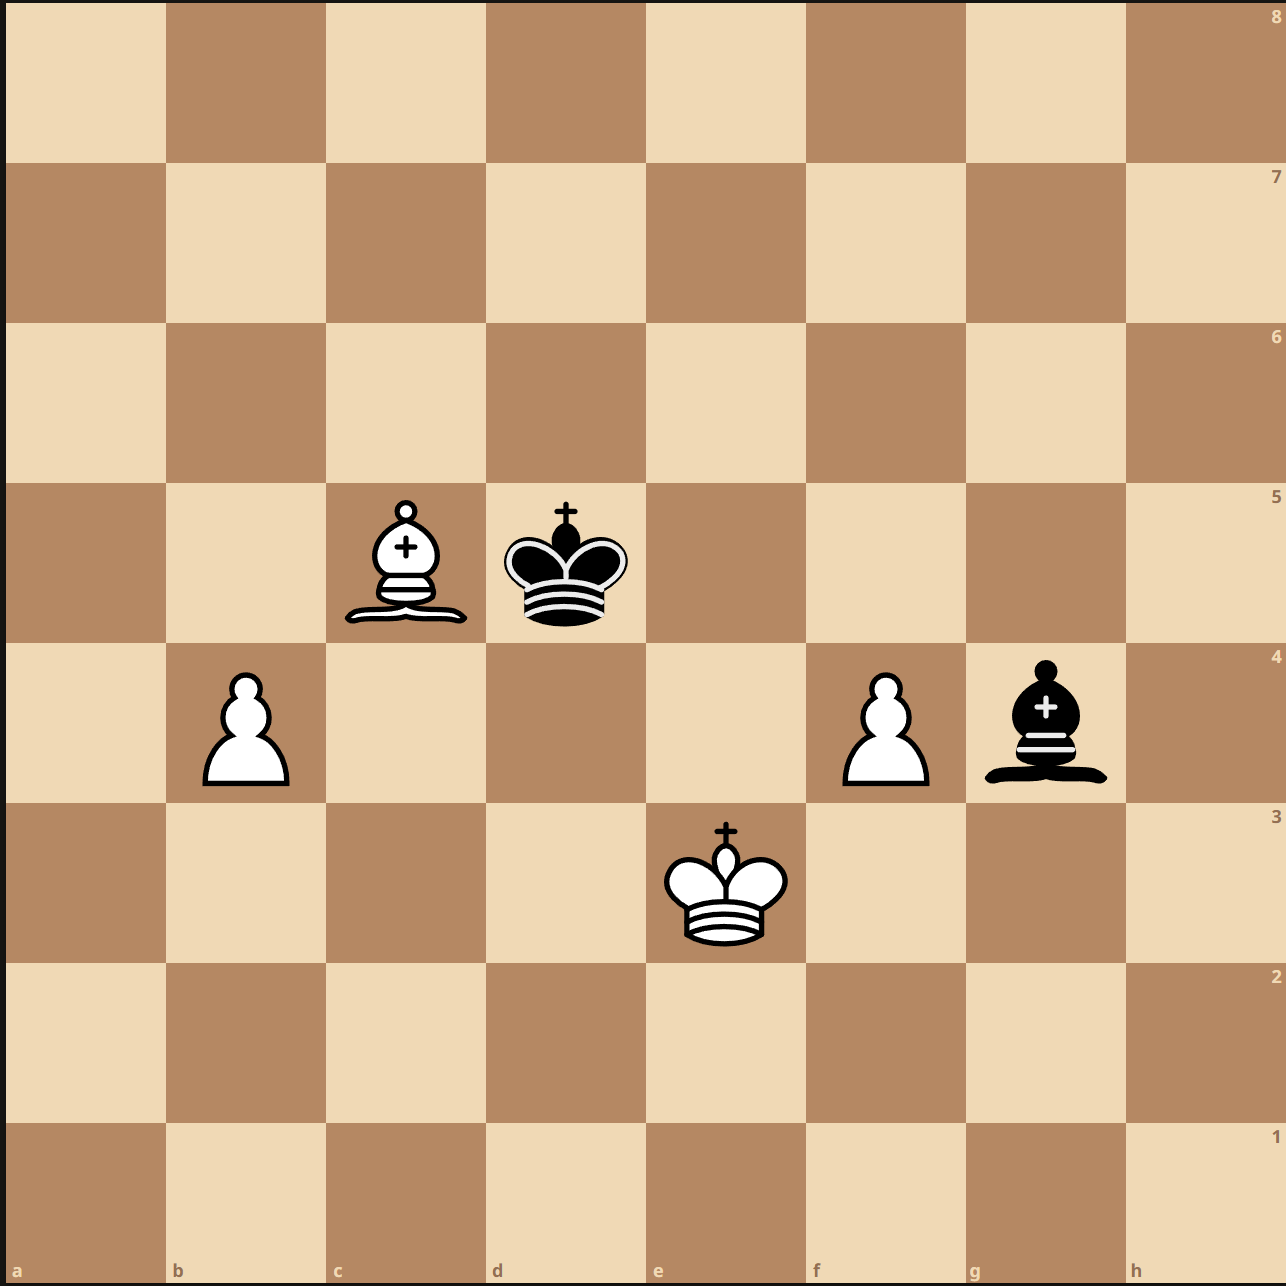
\includegraphics[width=\linewidth/3]{board.png}
    \caption{Scacchiera nella classica posizione di finale con alfieri di colore opposto }
    \label{board}
\end{figure}
\newpage
\vfill
\begin{figure}
    \centering
    
\includegraphics[scale=0.2]{placeholder.png}
    \caption{Rappresentazione set-wise della scacchiera in figura \ref{board} }
\end{figure}

\vfill
\clearpage


\section{Rappresentazione della scacchiera Casellocentrica}
La rappresentazione casellocentrica  mantiene un associazione inversa rispetto a quella pezzocentrica,
per ogni casella conserviamo in memoria se è vuota o occupata da un pezzo in particolare.
La macro-categoria di  rappresentazione più comune è la Mailbox:

\subsubsection{Mailbox}
La rappresentazione Mailbox è una rappresentazione casellocentrica dove la codifica di ogni casella risiede in una struttura dati
che permette l'accesso casuale ,solitamente si utilizza un array con l'indice che codifica dal numero della casella in array monodimensionali
o dalla coppia traversa/colonna\footnote{termini scacchistici per indicare le righe e le colonne della scacchiera} in array bidimensionali.
Il nome deriva dall'associazione di ogni indice al concetto di "indirizzo" di una casella postale.Le implementazioni più famose e
comuni del concetto di Mailbox sono la 8x8 Board e la 10x12 Board.

\subsubsection{8x8 Board}
Una board 8x8,figura \ref{otto} è una rappresentazione pezzocentrica consistente o in un array bidimensionale di bytes o interi, contenenti rappresentazioni codificate
per i pezzi e per la casella vuota, con i due indici ricavati dalla coppia traversa/colonna che identifica la casella sulla scacchiera ,
o più comunemente un array monodimensionale con indici da 0 a 63,uno per ogni casella della scacchiera.
Questo tipo di rappresentazione è usata spesso come rappresentazione ridondante all'interno di programmi che utilizzano bitboards
per individuare se e quali pezzi sono presenti su una casella in maniera efficiente.
\begin{figure}[!ht]
    \centering
    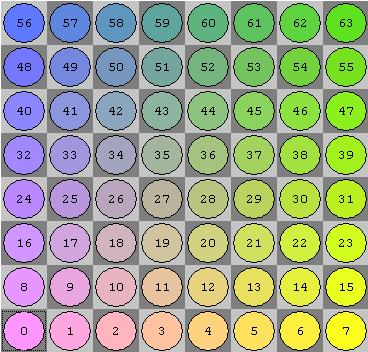
\includegraphics[width=\linewidth/2]{8x8 board.png}
    \caption{board numbering}
    \label{otto}
\end{figure}

\subsubsection{10x12 Board}
Una board 10x12  contorna una  board 8x8   con traverse e colonne sentinelle  per individuare  indici al di fuori della scacchiera durante la generazione delle mosse
\vfill
\begin{figure}[!ht]
    \centering
    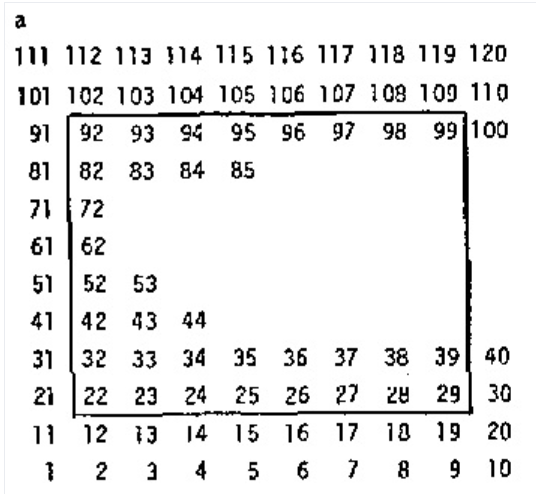
\includegraphics[width=\linewidth/2]{10x12 board.png}
    \caption{Rappresentazione di una board 10x12,notare come le 2 traverse extra sopra e sotto siano necessarie per evitare accessi out of bounds in caso di cavalli posizionati sulla prima o ottava fila }
\end{figure}
\vfill
\clearpage


\section{Rappresentazione dei pezzi}
una volta scelto il tipo di rappresentazione della scacchiera si può iniziare a pensare alla rappresentazione dei pezzi,
anche se può sembrare controintuitivo i pezzi non hanno bisogno di una struttura elaborata,la generazione delle possibili
mosse verrà gestita nella move generation ed il loro spostamento all'interno della scacchiera verrà gestito dalla funzione
MakeMove (approfondimenti riguardo questi due argomenti verranno presto forniti),per i pezzi quindi abbiamo bisogno di una
rappresentazione semplice, di facile interpretazione e che occupi poco spazio,rappresentazioni molto comuni sono quella
tramite interi, dove ad ogni tipo di pezzo viene assegnato un numero che funge da identificativo univoco e quella tramite
caratteri, dove ad ogni tipo di pezzo viene assegnato un carattere che lo identifica.


\section{Esempio di implementazione}
Nel motore che andremo a realizzare verrà adottato un approccio ibrido,con bitboards utilizzate per conservare le posizioni dei pedoni,una board 10x12 per tenere traccia di tutti i pezzi in gioco
e delle piece-lists per effettuare più rapidamente operazioni di lookup, la codifica dei pezzi avverrà tramite l'utilizzo di interi e il linguaggio utilizzato come già specificato precedentemente  sarà il C.

\subsubsection{Codifica dei pezzi} \label{codifica}
La codifica dei pezzi è realizzata tramite interi,per un uso più agevole all'interno del codice però, si consiglia la realizzazione
di un enum col quale mappare gli interi a dei simboli più facili da ricordare mnemonicamente.Si approfitta di questa sezione anche per introdurre
ulteriori enum utili per descrivere costanti all'interno del motore.
\begin{figure}[!ht]
    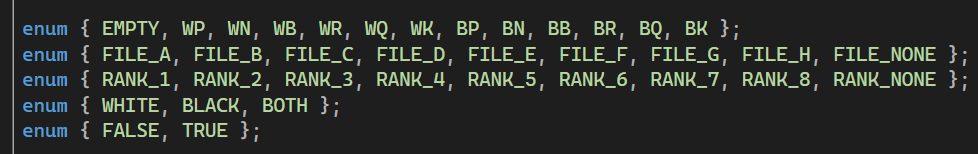
\includegraphics[width=\linewidth]{enums.png}
    \caption{set di enum consigliato per lo svolgimento di questo progetto }
    \label{enums}
\end{figure}

Inoltre,essendo un motore scacchistico un progetto che predilige la rapidità di esecuzione più di ogni altra cosa,
anche se sconsigliabile in quasi ogni altro contesto,conserviamo i dati che caratterizzano i pezzi,sulla base del loro indice,in un insieme di array che verrà condiviso come insieme di variabili
esterne dall'intero progetto, permettendo un lookup in tempo costante di tali informazioni.Per fare ciò adoperiamo un file header che conterrà le dichiarazioni ed un unico file sorgente dove saranno presenti le
definizioni.Definiamo infine delle macro per rendere il codice più pulito e leggibile.
\begin{figure}[!tbp]
    \centering
    \begin{minipage}{0.4\textwidth}
        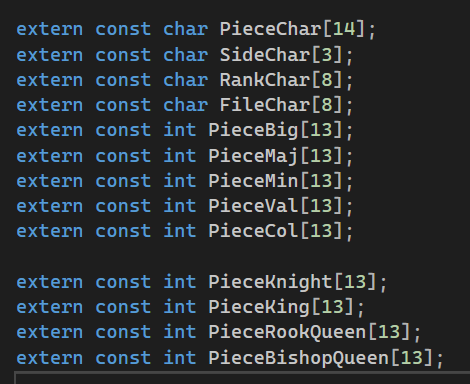
\includegraphics[width=\textwidth]{PieceDatah.png}
        \caption{PieceData.h}
    \end{minipage}
    \hfill
    \begin{minipage}{0.4\textwidth}
        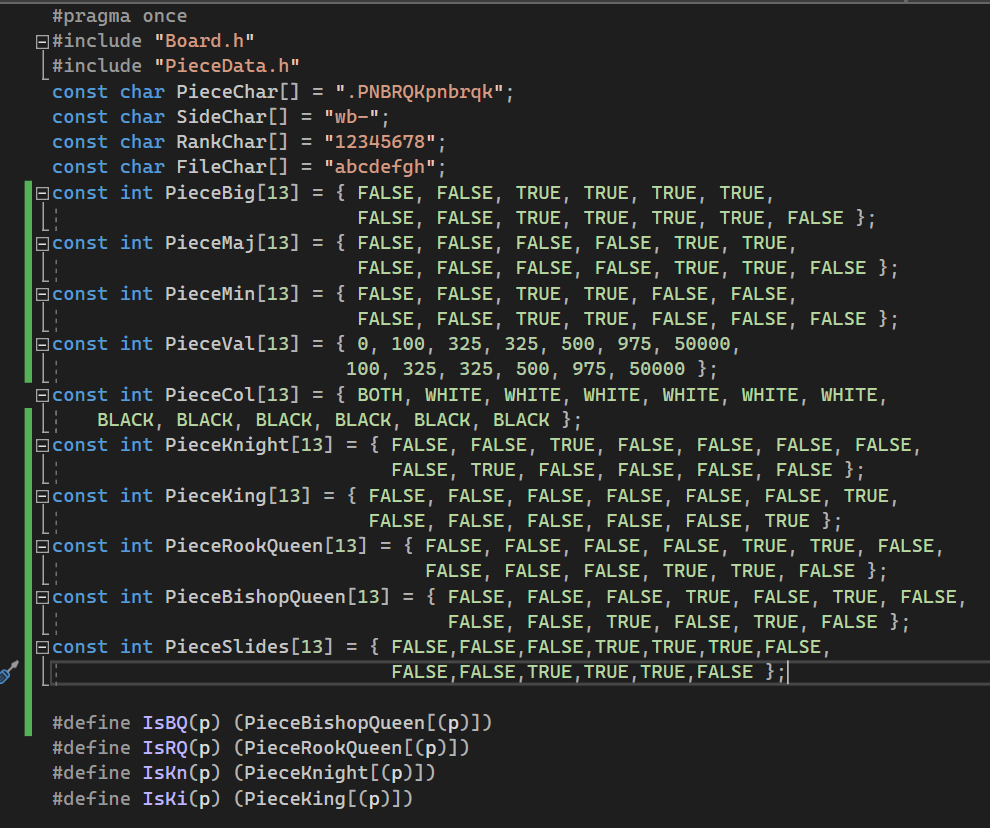
\includegraphics[width=\textwidth]{PieceDatac.png}
        \caption{PieceData.c}
    \end{minipage}
\end{figure}



\subsubsection{Realizzare una bitboard}
Come precedentemente spiegato, una bitboard non è altro che una parola di 64 bit,
utilizzando il linguaggio C ci basta definire una Bitboard come un unsigned long long int come nella figura \ref{bitboard.h} riga 2.
Oltre alla dichiarazione del tipo bitboard possiamo notare la dichiarazione di alcune funzioni indispensabili per operare sulla stessa,
le firme sono disponibili nella figura \ref{bitboard.h} ,mentre nella figura \ref{fig:bitboard.c} possiamo vedere delle implementazioni di esempio.
Nella figura \ref{bitboard.h} troviamo anche due macro, SETBIT e CLRBIT,che settano ad 1 o 0 uno specifico bit di una bitboard.



\vfill
\begin{figure}[!ht]
    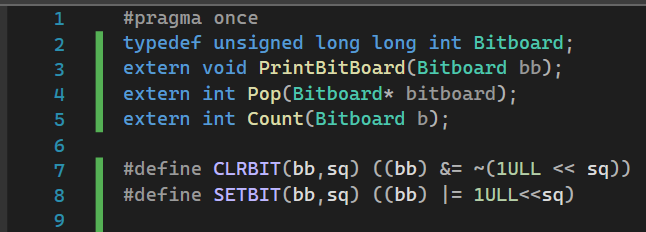
\includegraphics[width=\linewidth]{bitboard-h.png}
    \caption{ bitboard.h }
    \label{bitboard.h}
\end{figure}

\begin{figure}[H]
    \begin{minipage}[t]{.63\textwidth}
        \centering \raisebox{\dimexpr-\height+1.5ex\relax}{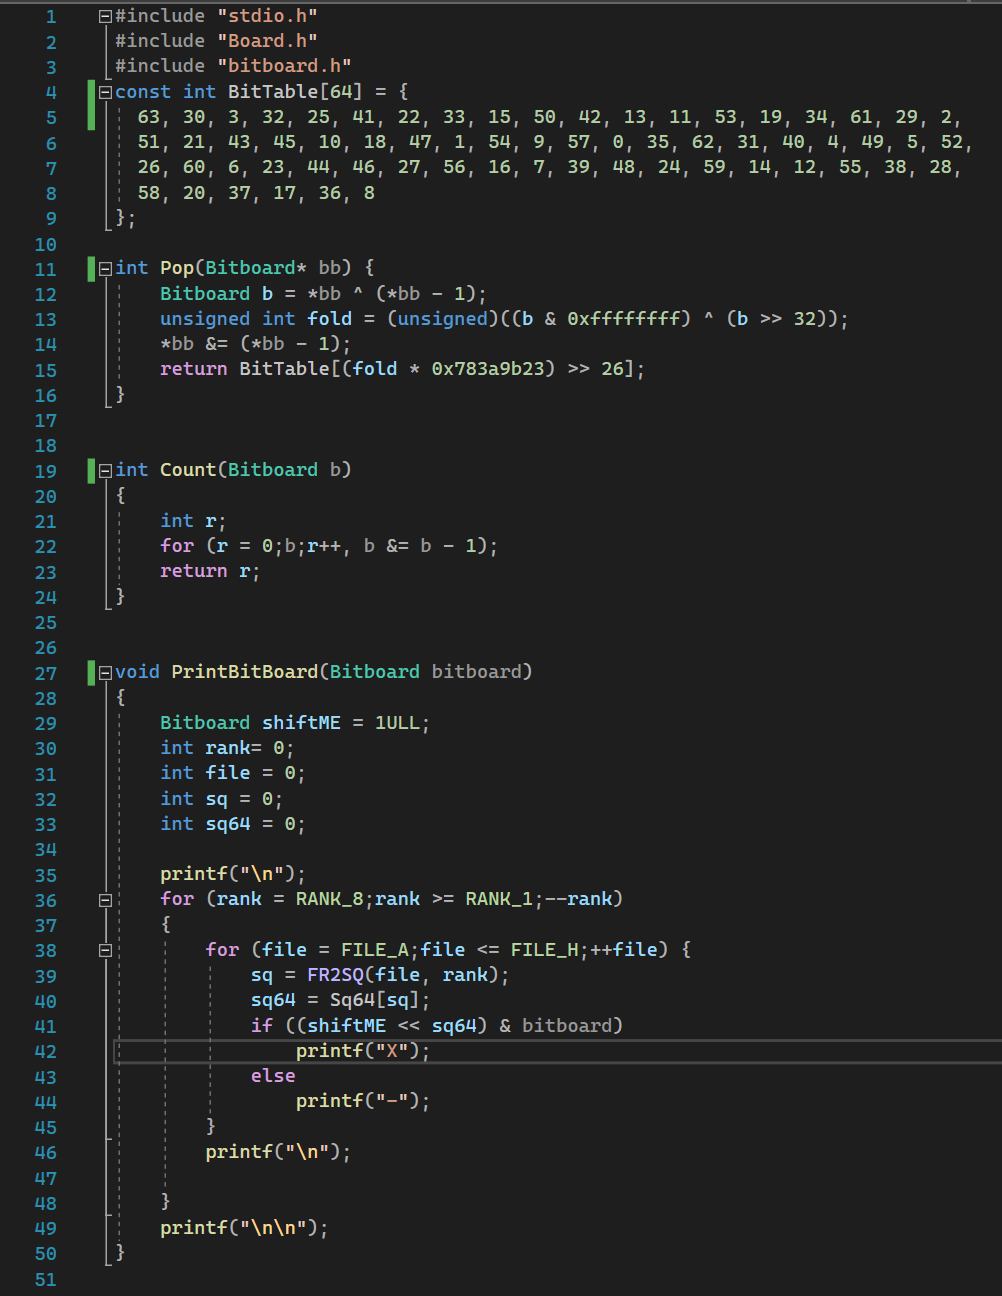
\includegraphics[scale=0.5]{bitboard-c.png}

        }
        \caption{bitboard.c}
        \label{fig:bitboard.c}
    \end{minipage}
    \begin{minipage}[t]{0.35\textwidth}
        {In particolare PrintbitBoard ci permette di visualizzare in output una bitboard,Pop restituisce l'indice del primo bit impostato a 1 nella bitboard
            (da meno a più significativo ) e  lo setta a 0 e Count restituisce il numero di bit settati a 1 di una bitboard.
            l'array BitTable è utilizzato per la fase di bitscan (la ricerca del primo bit settato ad 1 meno significativo)
            e risulta troppo complesso da spiegare in quella che è una guida introduttiva,per approfondire si consiglia
            la lettura della pagina sulla bitscan della ChessProgrammingWiki.
        }

    \end{minipage}
\end{figure}



\subsubsection{Realizzare la scacchiera}
Iniziamo con la definizione di alcune costanti che verranno utilizzate nella creazione della scacchiera:
\begin{figure}[!ht]
    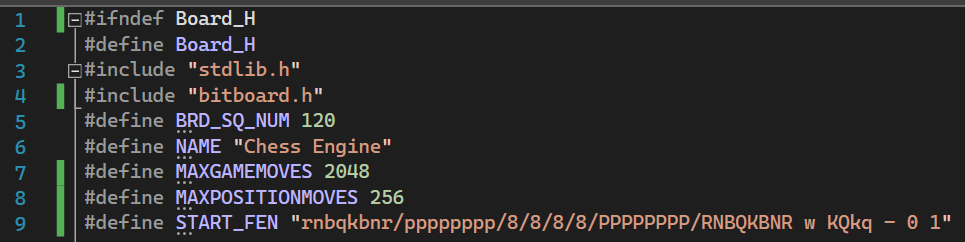
\includegraphics[width=\linewidth]{board-costants.png}
    \caption{ board-costants.png}
\end{figure}

\begin{itemize}
    \item \textbf{Include guard}:riga 1-2 direttiva rivolta al preprocessore usata nel file header per evitare problemi
          di doppia definizione in fase di linking.
    \item \textbf{Include(s)}: inclusione delle librerie necessarie alla realizzazione della scacchiera.
    \item \textbf{BRD\_SQ\_NUM}:numero di casella della scacchiera, nel caso di una rappresentazione 10x12 sono 120.
    \item \textbf{(NAME)}: Nome scelto per il motore scacchistico.
    \item \textbf{MAXGAMEMOVES}: Massimo numero di mosse in una partita,il numero più alto di mosse mai registrato si attesta intorno alle
          1000 mosse,2048 quindi è un buon limite .
    \item \textbf{(MAXPOSITIONMOVES)}: massimo numero di mosse eseguibili a partire da una singola posizione,è definibile anche come
          la massima profondità di ricerca a partire da un nodo N,dove il nodo N è una data posizione.
    \item \textbf{START\_FEN}: notazione Forsyth-Edwards di una scacchiera ad inizio partita,
          per approfondire si legga https://en.wikipedia.org/wiki/Forsyth-Edwards\_Notation.
\end{itemize}

Vediamo ora il codice che implementa la scacchiera,come detto nell'introduzione, la scacchiera oltre a contenere i pezzi
contiene anche le informazioni sullo stato delle partita,vedremo quindi anche come gestire questo tipo di dati.

\begin{figure}[H]
    \centering
    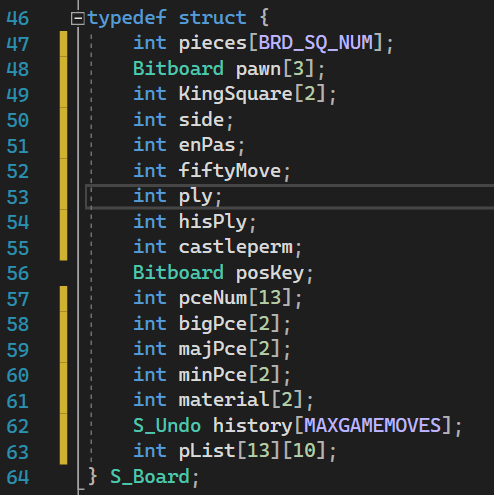
\includegraphics[width=\linewidth/2]{board-code.png}
    \caption{ board-code.png}
\end{figure}

\begin{itemize}
    \item \textbf{pieces}:è un array che per ogni casella della scacchiera memorizza  se c'è un pezzo, o se la casella è non valida (è quindi una delle caselle "sentinella" proprie della rappresentazione 10x12).
    \item \textbf{pawn}: è un array di 3 Bitboard per memorizzare la posizione dei pedoni bianchi,neri e di entrambi combinati.
    \item \textbf{KingSquare}:è un array che contiene la posizione del re bianco e del re nero,utile per velocizzare delle operazioni di lookup fondamentali in casi nei quali la posizione del re sulla scacchiera gioca
          un ruolo fondamentale.
    \item \textbf{side}: intero che codifica quale lato può muovere, gli indici si basano sul enum della figura \ref{enums}.
    \item \textbf{enPas}:intero che codifica se  è possibile una cattura en passant ed in quale casella, maggiori dettagli nel paragrafo \ref{enpassant}.
    \item \textbf{(fiftyMove)}: Contatore per la regola delle 50 mosse.
    \item \textbf{ply}: numero di semimosse   in una search instance
    \item \textbf{hisPly}:numero totale di semimosse.
    \item \textbf{castleperm}: intero che codifica i permessi di arrocco tramite una rappresentazione sotto forma di stringa di bit, maggiori dettagli nel paragrafo \ref{arrocco}
    \item \textbf{poskey}: chiave hash unica che codifica la posizione attualmente presente sulla scacchiera,utile per il controllo delle posizioni ripetute.
    \item \textbf{pceNum}: un array che restituisce il numero dei pezzi di quel tipo sulla scacchiera,con gli indici codificati  come nell'enum della figura \ref{enums},ie: pceNum[2] restituisce il numero di cavalli bianchi.
    \item \textbf{bigPce}: array che restituisce il numero di pezzi grandi\footnote{i pezzi cosiddetti "grandi" sono tutti i pezzi ad esclusione del pedone e del re} ancora in gioco  per entrambi i colori con gli indici codificati  come nell'enum della figura \ref{enums}.
    \item \textbf{majPce}:array che restituisce il numero di pezzi maggiori\footnote{i pezzi cosiddetti "maggiori" sono la regina e la torre} ancora in gioco  per entrambi i colori con gli indici codificati come nell'enum della figura \ref{enums}.
    \item \textbf{minPce}: array che restituisce il numero di pezzi minori\footnote{i pezzi cosiddetti "minori" sono il cavallo e l'alfiere} ancora in gioco  per entrambi i colori con gli indici codificati codificati come nell'enum della figura \ref{enums}.
    \item \textbf{material}: mostra il valore totale del materiale di ogni giocatore con gli indici codificati  come nell'enum della figura \ref{enums}.
    \item \textbf{history}: array di S\_Undo Struttura dati che contiene ogni mossa effettuata e lo stato della scacchiera prima che quella mossa venisse fatta,fondamentale per potere effettuare
          il rollback della scacchiera ad uno stato precedente, maggiori dettagli nel paragrafo \ref{undo}
    \item \textbf{pList}: un array bidimensionale  che per ogni tipo  pezzo memorizza la posizione di ogni istanza di quel pezzo, fino ad un massimo di 10 possibili istanze (il massimo teorico di copie di un pezzo negli scacchi è 10),
          il primo indice varia da 0 a 12 come nell'enum della figura \ref{enums}, e codifica ogni tipo possibile di pezzo,il secondo indice indica quale dei 10 pezzi possibili stiamo cercando,non è garantita nessuna forma
          di ordinamento.
\end{itemize}

Definiamo un enum per poter accedere alle caselle della scacchiera in maniera più naturale \ref{boardenum}
\begin{figure}[H]
    \centering
    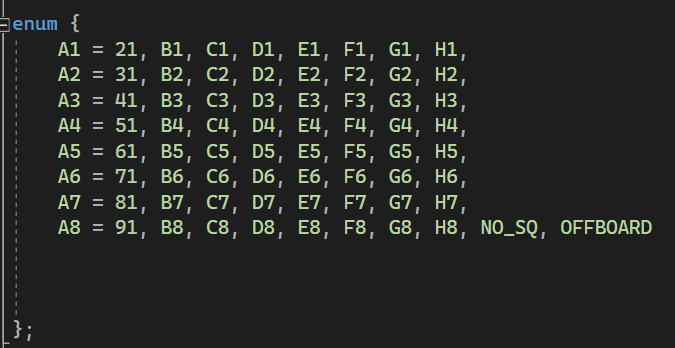
\includegraphics[width=\linewidth/2]{enumscacchiera.png}
    \caption{ board-enum.png}
    \label{boardenum}
\end{figure}

Infine definiamo,come visto nel paragrafo \ref{codifica}, degli array ai quali sarà possibile accedere globalmente,per effettuare in tempo costante il lookup delle conversioni dell'indice di una casella
da una rappresentazione 10x12 ad una 8x8 e viceversa, e della colonna e della traversa di appartenenza di una casella a partire dall'indice della stessa, la definizione è effettuata in Board\_Data.h mentre la definizione
è in init.c,una raccolta di funzioni che si occupano di inizializzare il programma all'avvio.

\begin{figure}
    \centering
    \begin{minipage}{0.3\textwidth}
        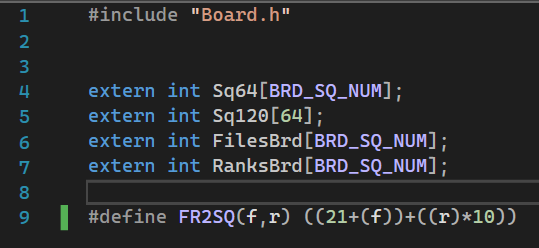
\includegraphics[width=\textwidth]{BoardData-h.png}
        \caption{Board\_Data.h}
    \end{minipage}
    \hfill
    \begin{minipage}{0.3\textwidth}
        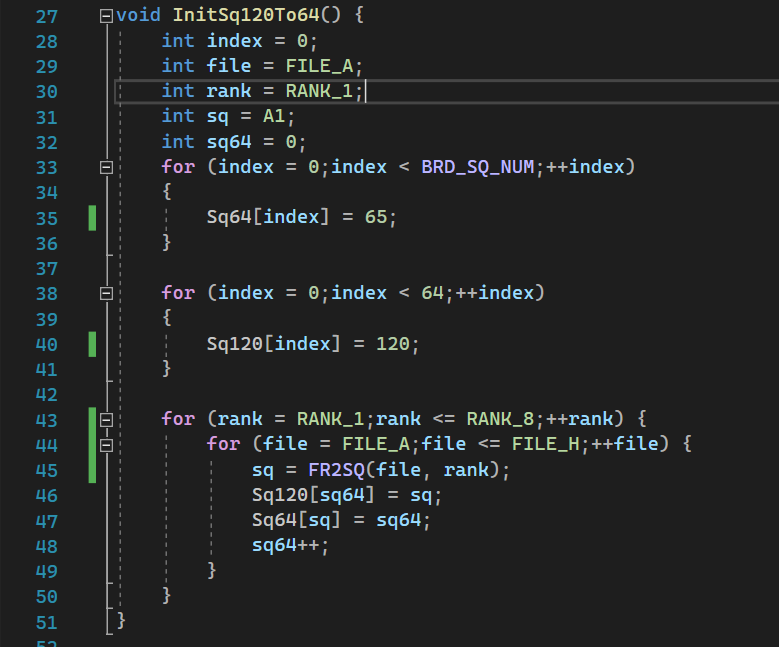
\includegraphics[width=\textwidth]{init1.png}
        \caption{init.c}
    \end{minipage}
    \hfill
    \begin{minipage}{0.3\textwidth}
        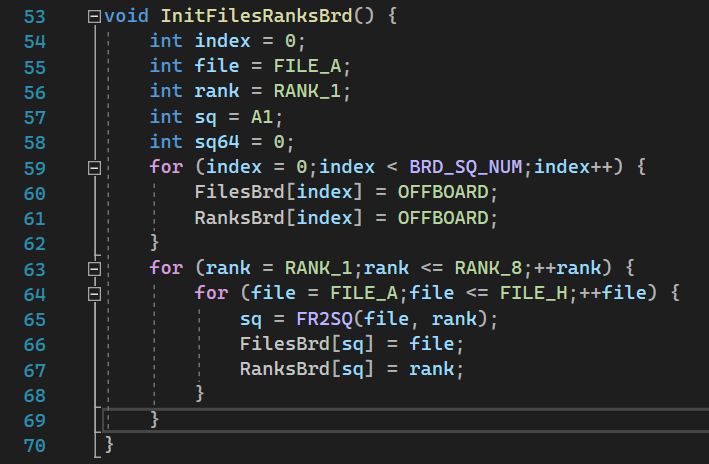
\includegraphics[width=\textwidth]{init2.png}
        \caption{init.c}
    \end{minipage}
\end{figure}



\subsubsection{Funzioni per operare sulla scacchiera}
Una volta definita la struttura della scacchiera è il momento di definire alcune funzioni indispensabili per operare sulla stessa,
nella figura \ref{scacchierah} troviamo le firme delle funzioni da porre nel file board.h,di seguito troviamo una descrizione dello scopo di ogni funzione e chiarimenti sulle implementazioni
\begin{figure}[H]
    \centering
    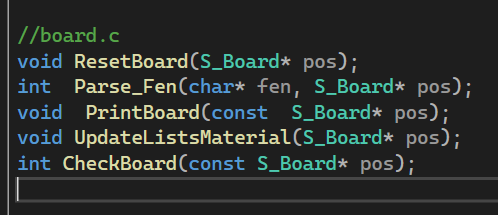
\includegraphics[width=\linewidth/2]{boardc.png}
    \caption{ board-h.png}
    \label{scacchierah}
\end{figure}


\subsubsection{ResetBoard}
\begin{figure}[H]
    \begin{minipage}[t]{.63\textwidth}
        \centering \raisebox{\dimexpr-\height+1.5ex\relax}{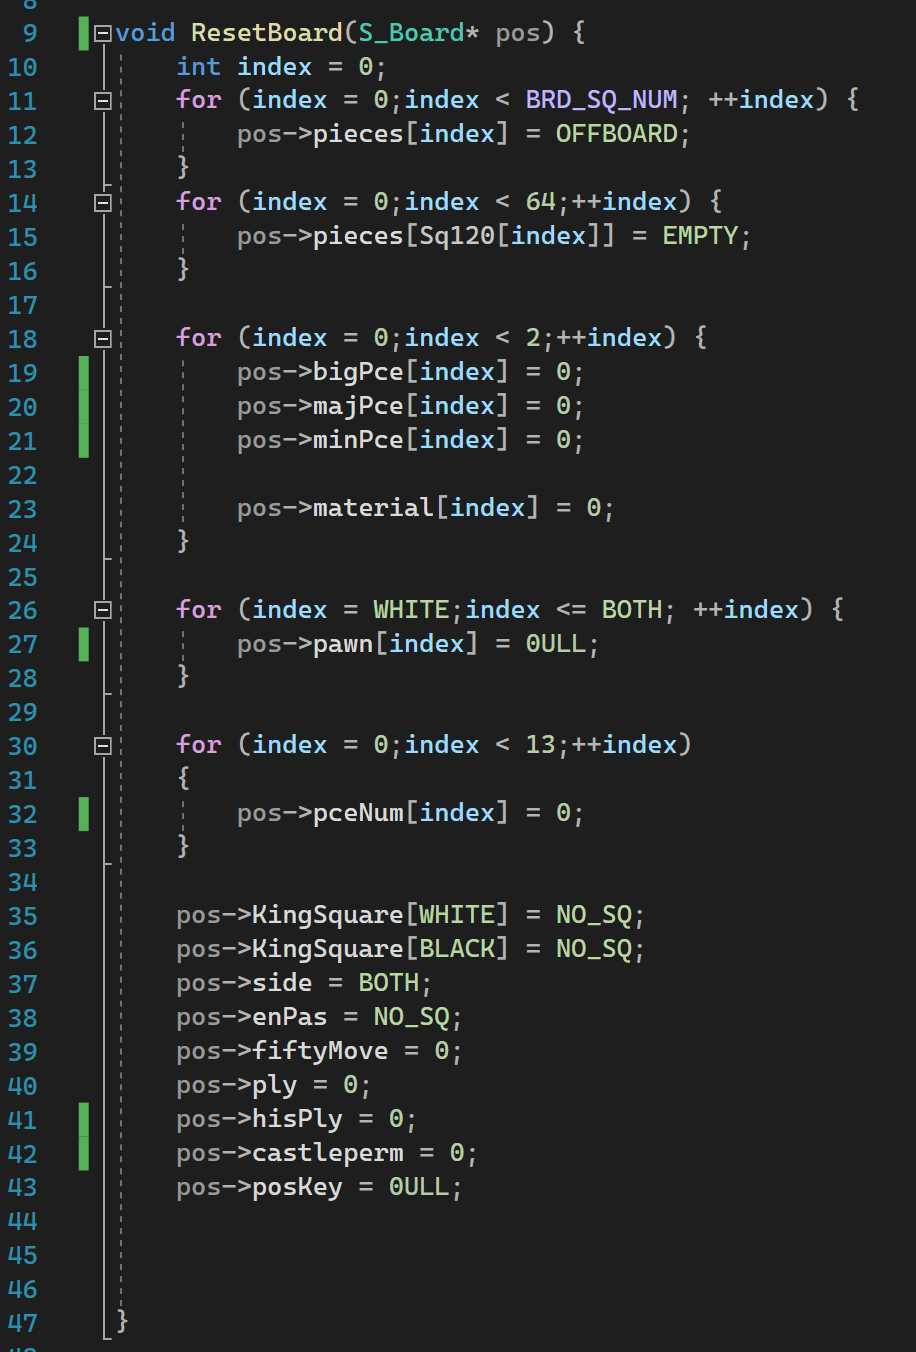
\includegraphics[scale=0.5]{ResetBoard.png}}
    \end{minipage}
    \begin{minipage}[t]{0.35\textwidth}
        \large{ResetBoard è la funzione che riporta la scacchiera ad uno stato neutro,prima ogni riquadro della scacchiera viene settato ad "offboard",il valore corrispondente ad una casella non valida,
            poi i riquadri appartenenti all'effettiva scacchiera,escluse quindi le caselle sentinella, vengono settate ad empty,in seguito abbiamo l'azzeramento di tutti i valori conservati dalla posizione}
    \end{minipage}
\end{figure}



\subsubsection{PrintBoard}
\begin{figure}[H]
    \begin{minipage}[t]{.63\textwidth}
        \centering \raisebox{\dimexpr-\height+1.5ex\relax}{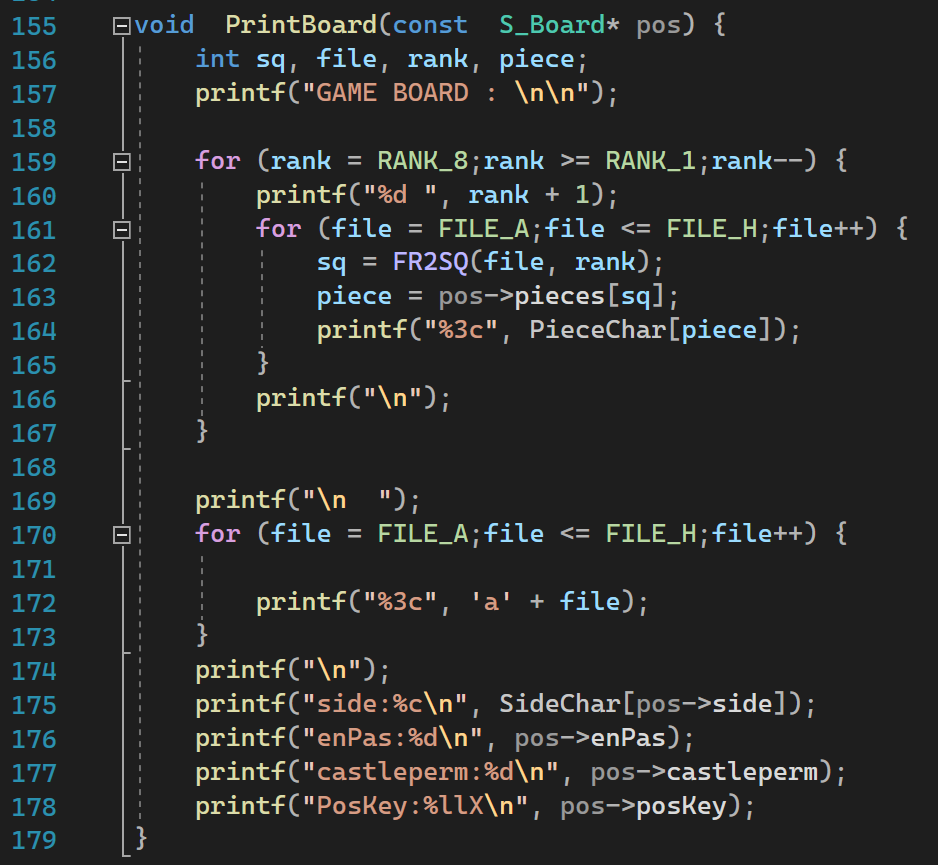
\includegraphics[scale=0.5]{PrintBoard.png}}
    \end{minipage}
    \begin{minipage}[t]{0.35\textwidth}
        \small{PrintBoard è la funzione che permette di visualizzare una scacchiera in stdout,ciclando per ogni casella viene mostrato l'eventuale pezzo presente ed in caso di casella vuota il carattere "." ,infine
            vengono mostrare le informazioni riguardanti la posizione, quali key univoca che la identifica,stato dei permessi di arrocco etc.}
    \end{minipage}
\end{figure}



\subsubsection{UpdateListMaterial}
\begin{figure}[H]
    \begin{minipage}[t]{.63\textwidth}
        \centering \raisebox{\dimexpr-\height+1.5ex\relax}{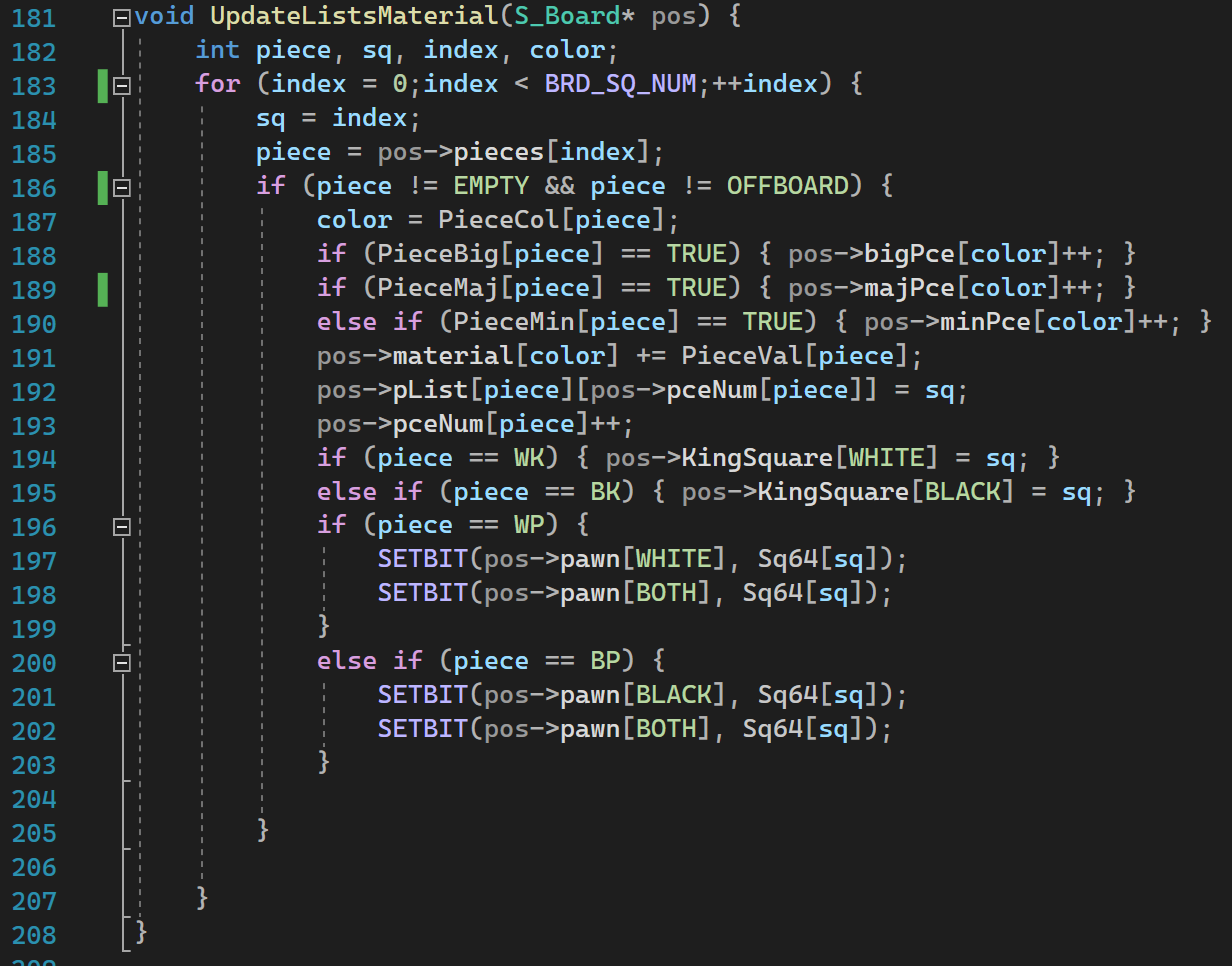
\includegraphics[scale=0.45]{UpdateListMaterial.png}}
    \end{minipage}
    \begin{minipage}[t]{0.35\textwidth}
        \small{UpdateListMaterial è la funzione che,data una scacchiera dal quale ricavare i dati della posizione,aggiorna in memoria lo stato della posizione,per ogni casella controlla l'eventuale presenza di pezzi,e,
            nel caso in cui trovi un pezzo,aggiorna tutte le variabili collegate ad esso,in particolare si segnala come per il re venga aggiornato KingSquare e per i pedoni vi sia un aggiornamento delle bitboard}
    \end{minipage}
\end{figure}


\subsubsection{ParseFen}


\begin{figure}[H]
    \centering
    \begin{minipage}[b]{0.4\textwidth}
        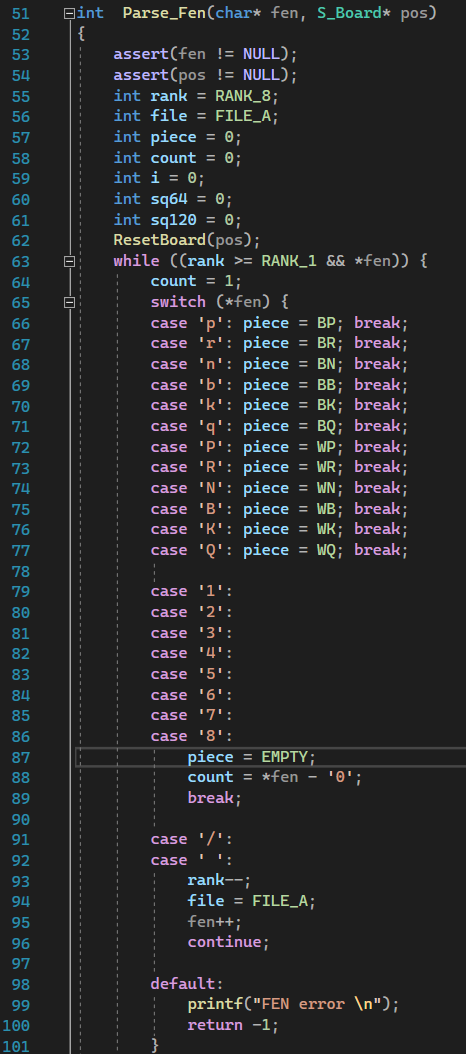
\includegraphics[width=\textwidth]{ParseFen1.png}
        \caption{ParseFen parte 1}
    \end{minipage}
    \hfill
    \begin{minipage}[b]{0.4\textwidth}
        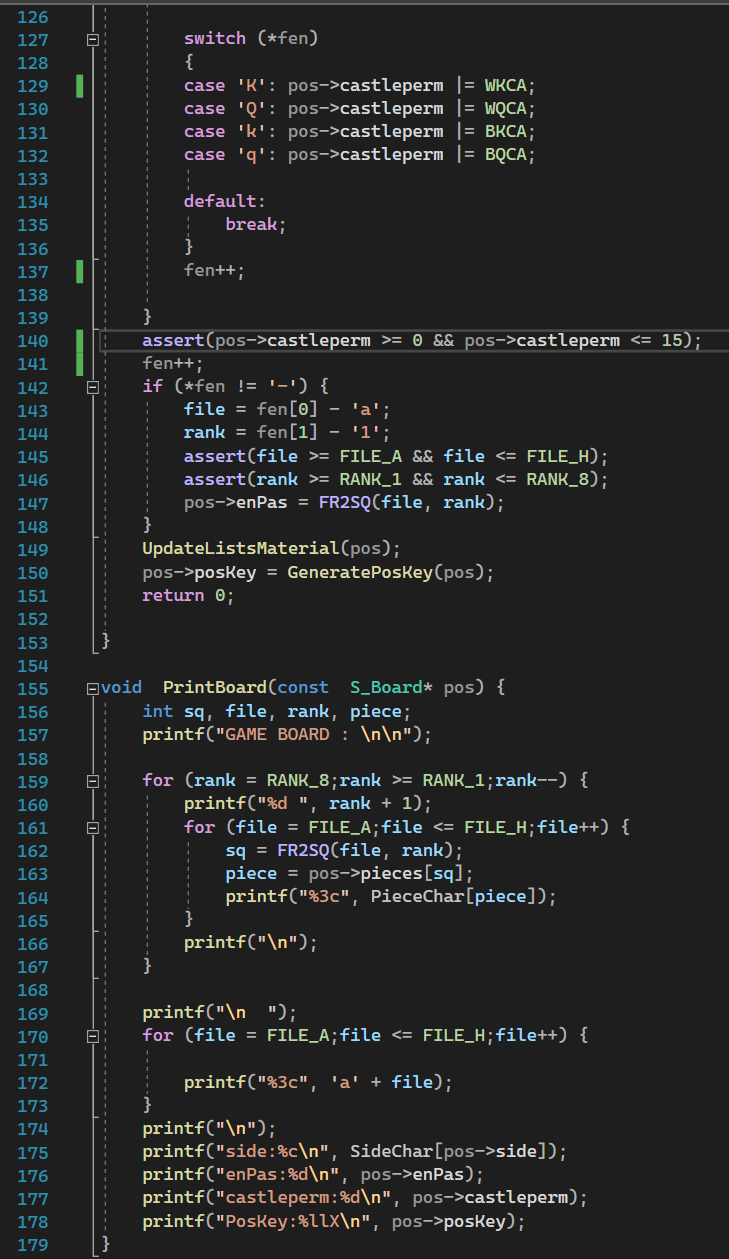
\includegraphics[width=\textwidth]{ParseFen2.png}
        \caption{ParseFen parte 2}
    \end{minipage}
\end{figure}





\section{Permessi di arrocco}
\label{arrocco}
L'arrocco è  una mossa particolare nel gioco degli scacchi che coinvolge il re e una delle due
torri. È l'unica mossa che permette di muovere due pezzi contemporaneamente nonché l'unica
in cui il re si muove di due caselle,Consiste nel muovere il re di due caselle a destra o a sinistra in direzione di una delle due torri e successivamente muovere la torre
(quella verso la quale il re si è mosso) nella casella compresa tra quelle di partenza e di arrivo del re.
Per indicare l'intenzione di effettuare un arrocco si deve prima sollevare il re e muoverlo di due case e solo successivamente muovere la torre nella casa di destinazione. Se si tocca la torre per prima si
deve effettuare, secondo la regola che il pezzo toccato dev'essere mosso, una mossa con la sola torre. Se si arrocca muovendo o toccando contemporaneamente il re e la torre, si commette una mossa illegale.
La mossa può essere effettuata solo se si è in presenza delle seguenti condizioni:
\begin{itemize}
    \item   il giocatore non ha mai mosso il re;
    \item il giocatore non ha mai mosso la torre coinvolta nell'arrocco;
    \item   non ci sono pezzi tra il re e la torre coinvolta;
    \item il re e la torre devono trovarsi sulla stessa traversa;
    \item  il re non deve essere sotto scacco;
    \item   il re, durante il movimento dell'arrocco, non deve attraversare caselle in cui si troverebbe sotto scacco.
    \item  L'arrocco non è vietato se ad essere sotto attacco (prima, durante o al termine della mossa) è la torre.
\end{itemize}
È inoltre permesso effettuare un arrocco anche qualora il re sia stato sotto scacco in precedenza e, ovviamente, non sia stato ancora mosso.

\begin{figure}[!tbp]
    \centering
    \begin{minipage}[b]{0.4\textwidth}
        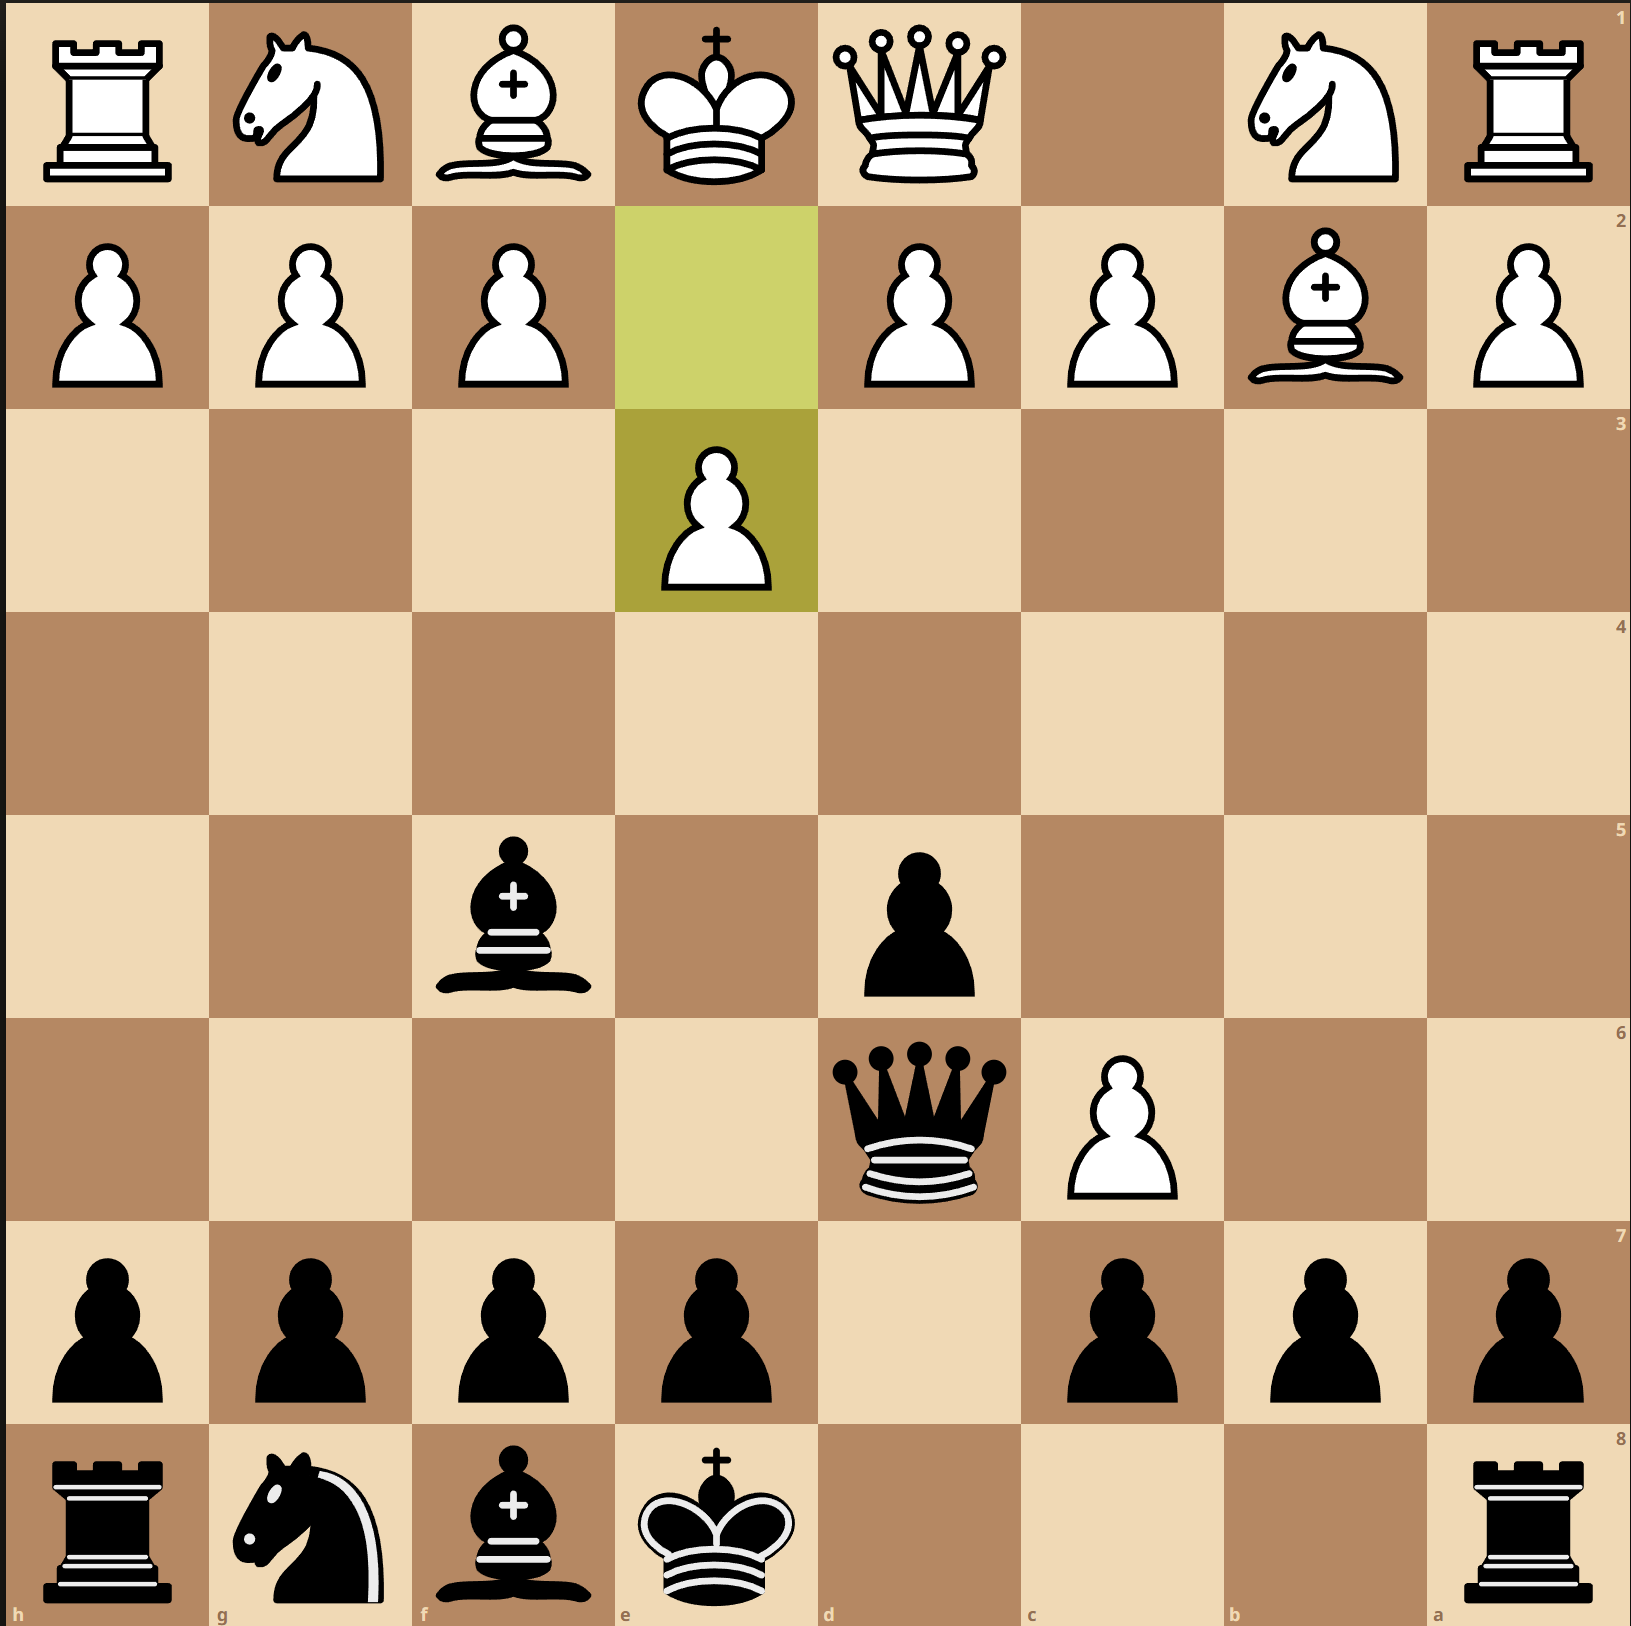
\includegraphics[width=\textwidth]{pre_arrocco.png}
        \caption{posizione di gioco dove è possibile arroccare}
        \label{prearrocco}
    \end{minipage}
    \hfill
    \begin{minipage}[b]{0.4\textwidth}
        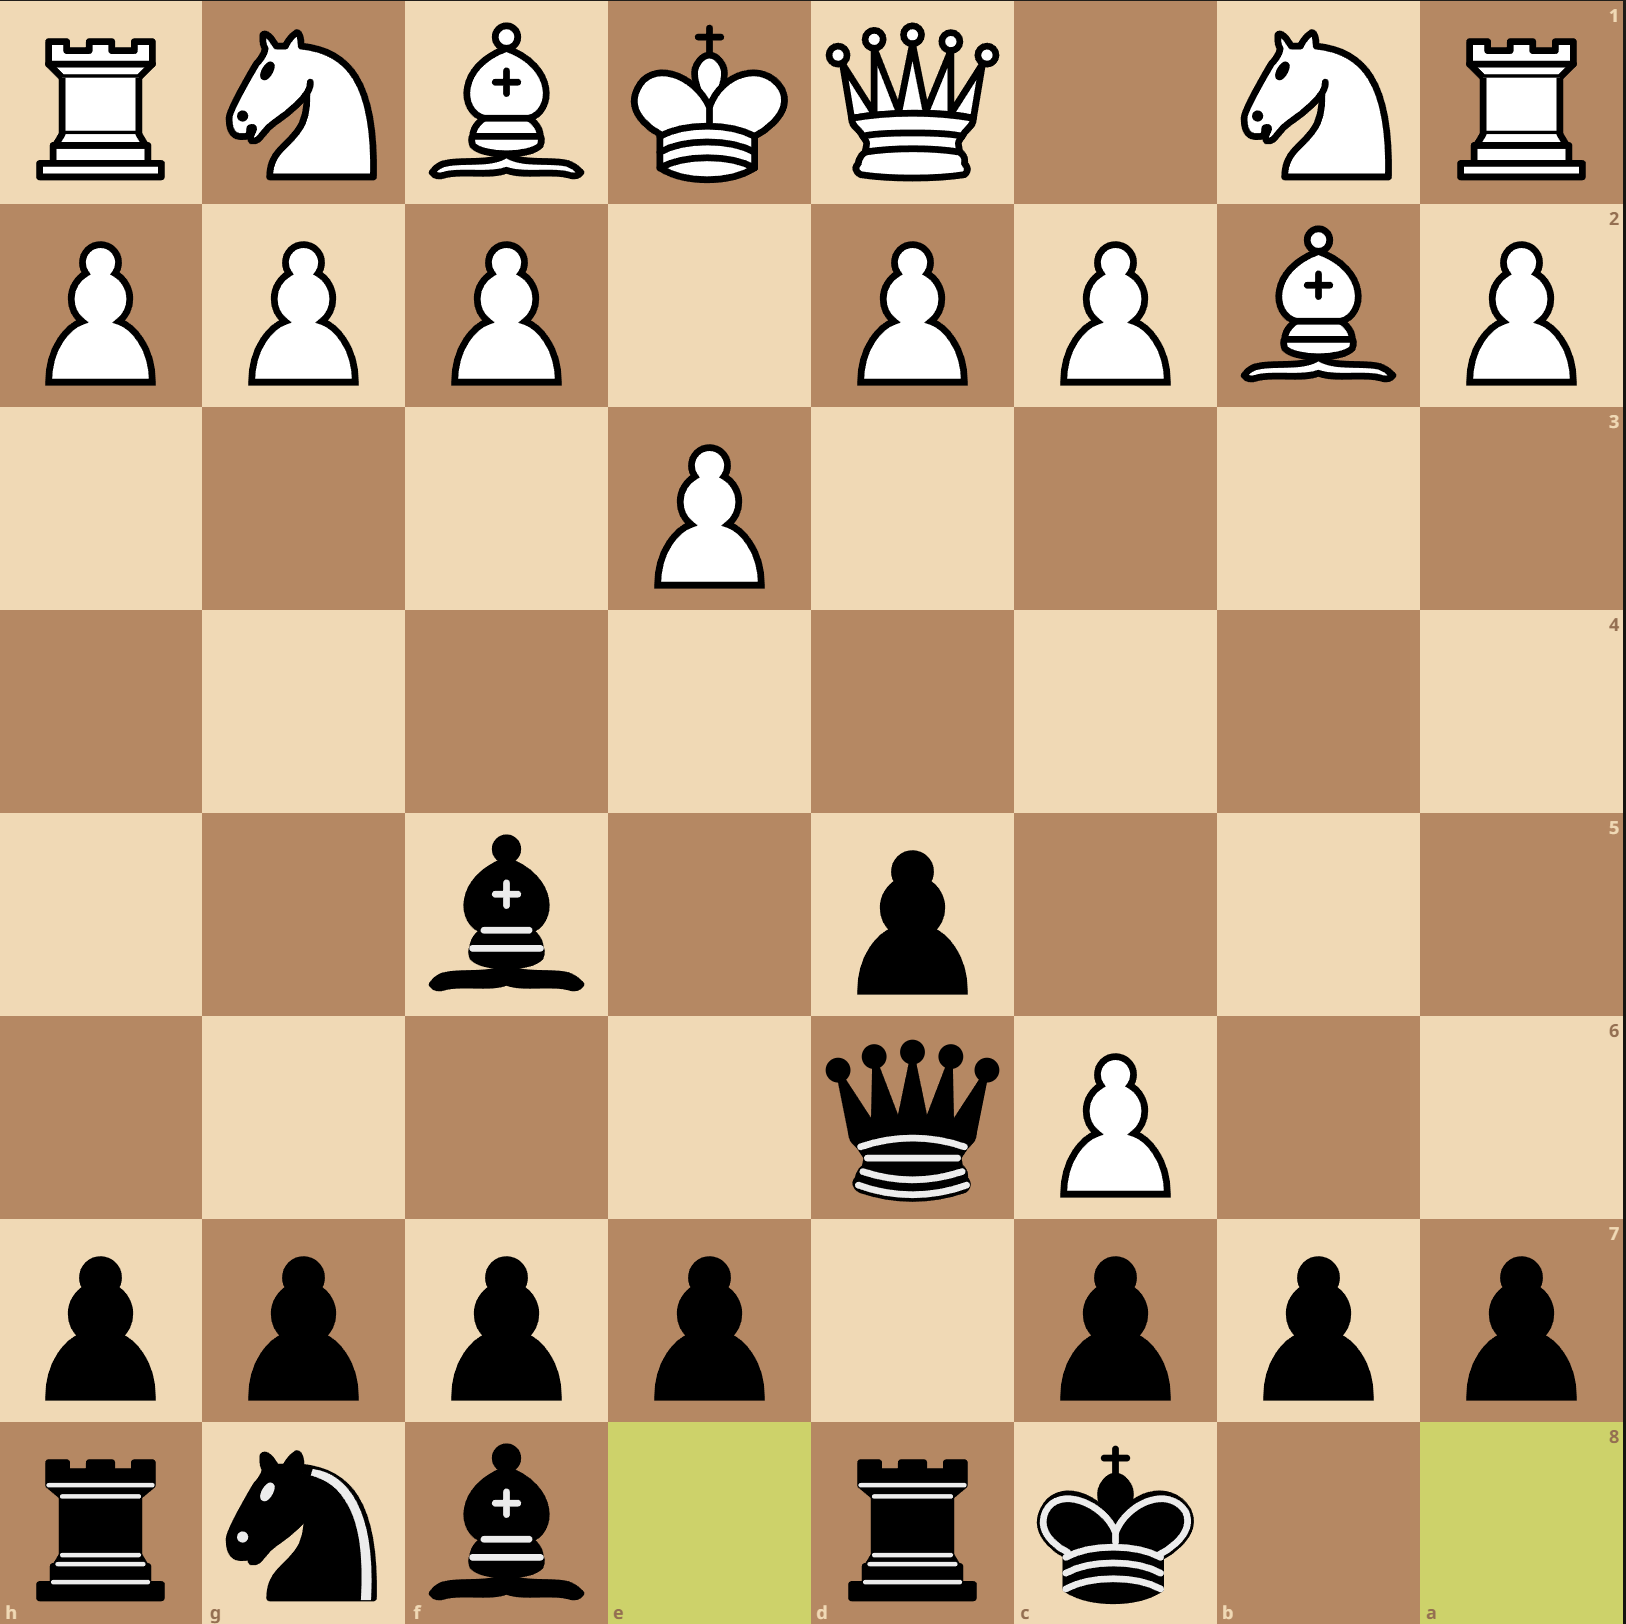
\includegraphics[width=\textwidth]{post_arrocco.png}
        \caption{posizione della figura \ref{prearrocco} post arrocco}
    \end{minipage}
\end{figure}

In totale sono possibili 4 arrocchi,re bianco dal lato della regina, re bianco dal lato del re, re nero dal lato della regina
re  nero dal lato del re \footnote{il lato del re è il lato dove si  trova il re rispetto alla regina all'inizio della partita
    equivale a destra per il bianco e sinistra per il nero, il lato della regina è il lato opposto},
volendo quindi codificare ogni permesso con un bit, la rappresentazione di tutti  i permessi è possibili utilizzando
una stringa di 4 bit,la variabile castleperm varrà quindi 1111 (15) se sono possibili tutti i 4  arrocchi,0000 se non sarà  possibile
effettuare nessuno dei 4 arrocchi, ed assumerà valori intermedi per indicare permessi che si trovano nel mezzo.\newline Si sottolinea che il permesso di arrocco
non è la possibilità di poter effettuare un arrocco in quel preciso momento della partita ma indica la possibilità in generale di poter effettuare un arrocco
nel caso in cui si verifichino le altre condizioni necessarie.\newline
In termini pratici la realizzazione si riduce cosi ad un enum { WKCA = 1, WQCA = 2, BKCA = 4, BQCA = 8 },
la variabile castleperm sarà inizializzata sempre a 15 dato che ad inizio della partita tutti gli arrocchi saranno sempre possibili,e,
per controllare o eliminare i permessi basterà usare delle operazioni bitwise.



\section{En passant}
\label{enpassant}
Nel gioco degli scacchi la presa en passant o presa al varco è una mossa speciale, cioè un'eccezione alle normali regole del movimento dei pezzi.
La presa en passant  è una mossa che coinvolge esclusivamente i pedoni e può essere eseguita da ciascun pedone che si trovi nelle condizioni adatte.
ed è legata alla caratteristica del pedone di spostarsi di due caselle quando viene mosso per la prima volta.
Quando un pedone, muovendosi di due passi (quindi per la prima volta), finisce esattamente accanto (sulla stessa traversa e su colonna adiacente) ad un pedone avversario,
nella mossa successiva quest'ultimo può catturarlo come se si fosse mosso di un passo solo.
È importante notare che, quando un pedone ha la possibilità di effettuare una presa en passant nei confronti di un pedone avversario, deve realizzarla subito, al verificarsi della posizione,
altrimenti perde il diritto a farlo.

\begin{figure}[H]
    \centering
    \begin{minipage}[b]{0.4\textwidth}
        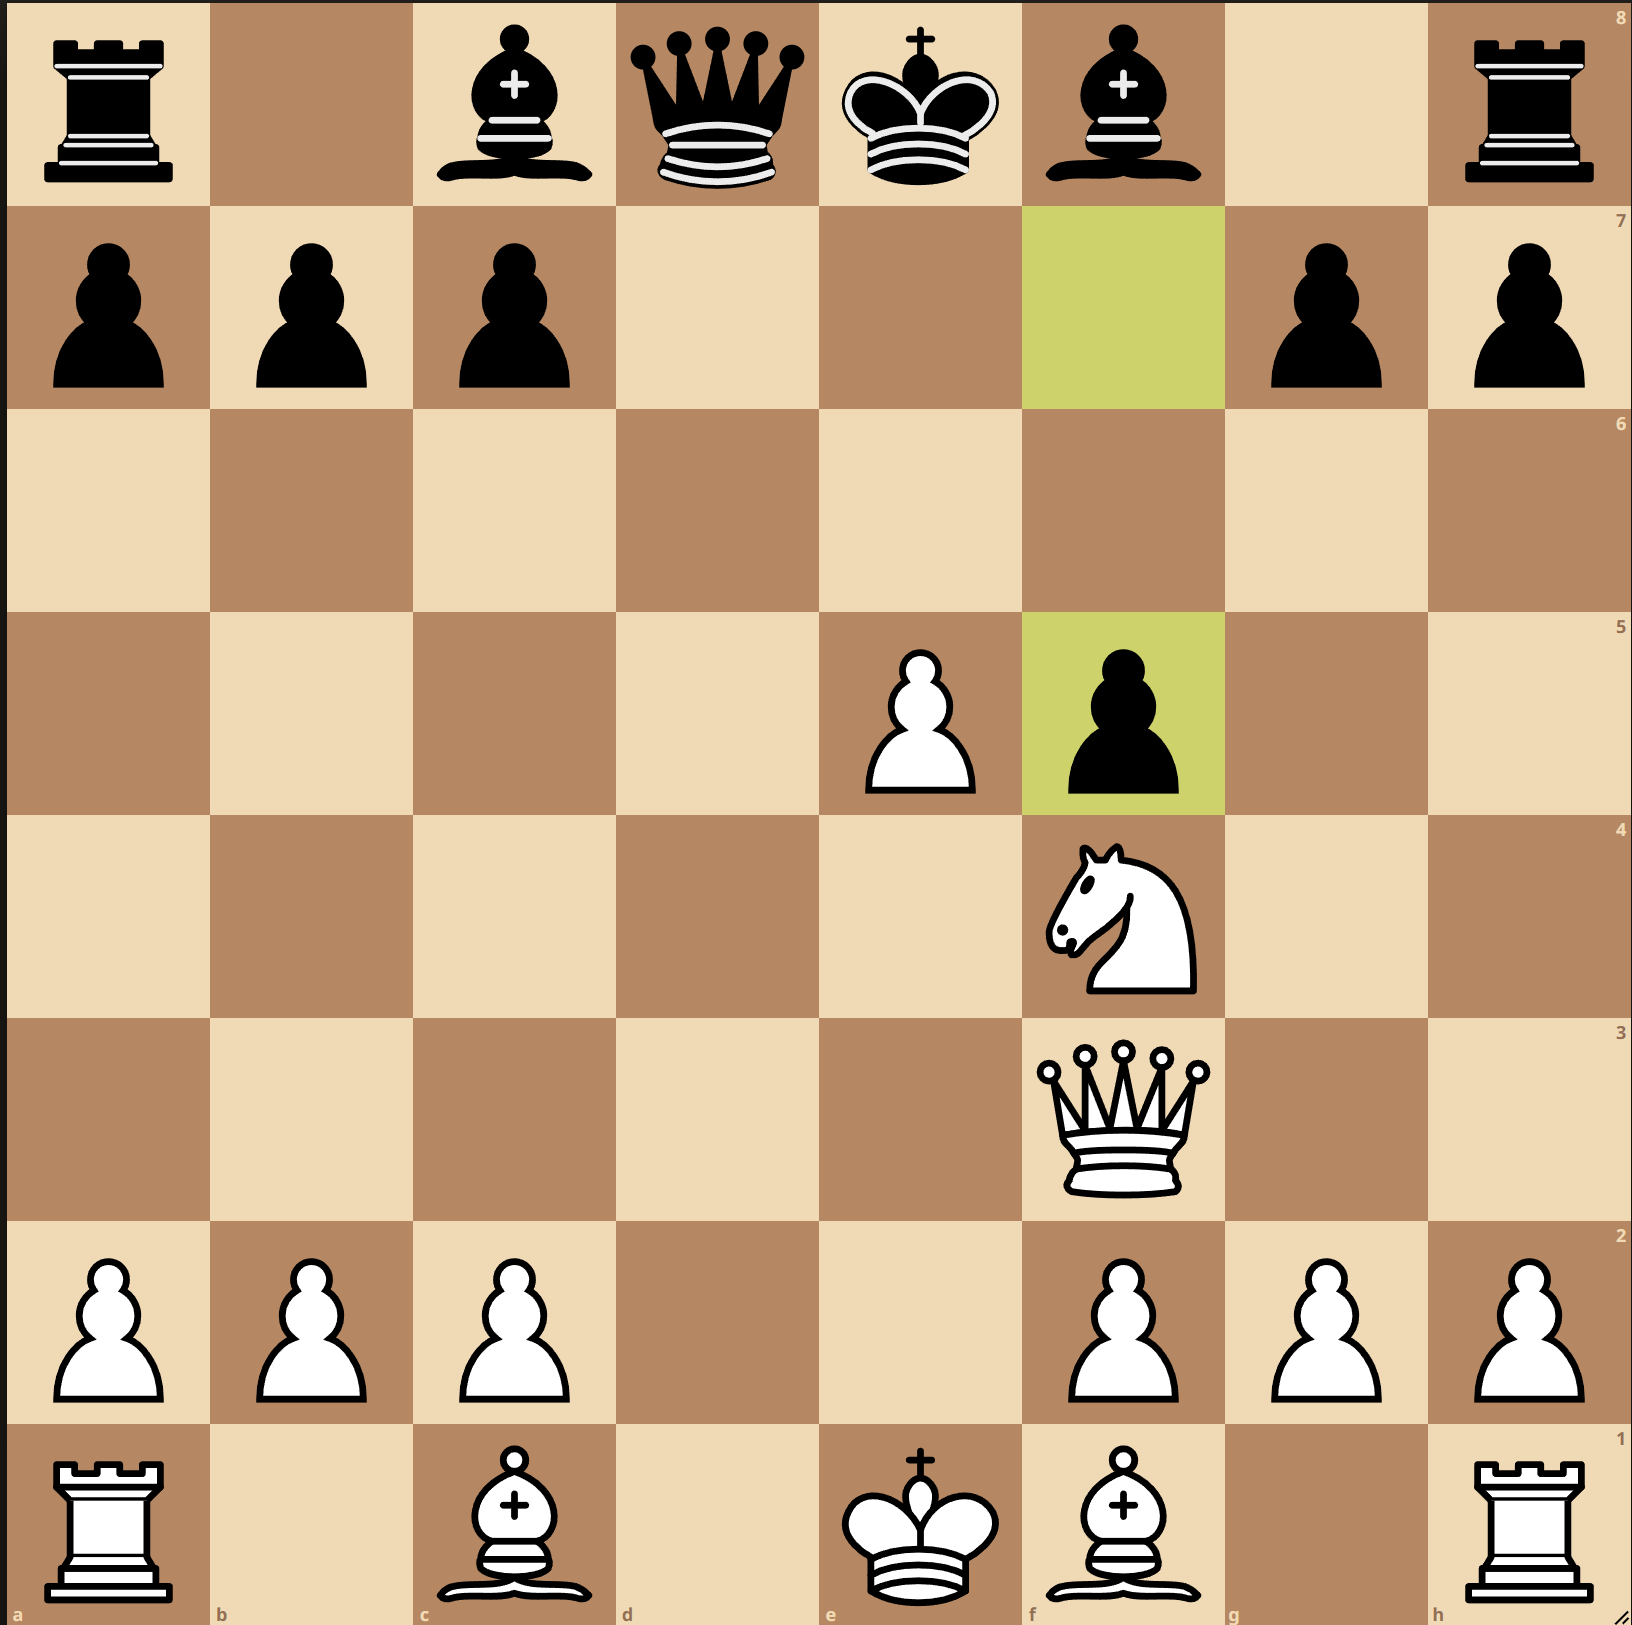
\includegraphics[width=\textwidth]{pre_enpas.png}
        \caption{posizione di gioco dove è possibile catturare con en passant}
        \label{pre_enpas}
    \end{minipage}
    \hfill
    \begin{minipage}[b]{0.4\textwidth}
        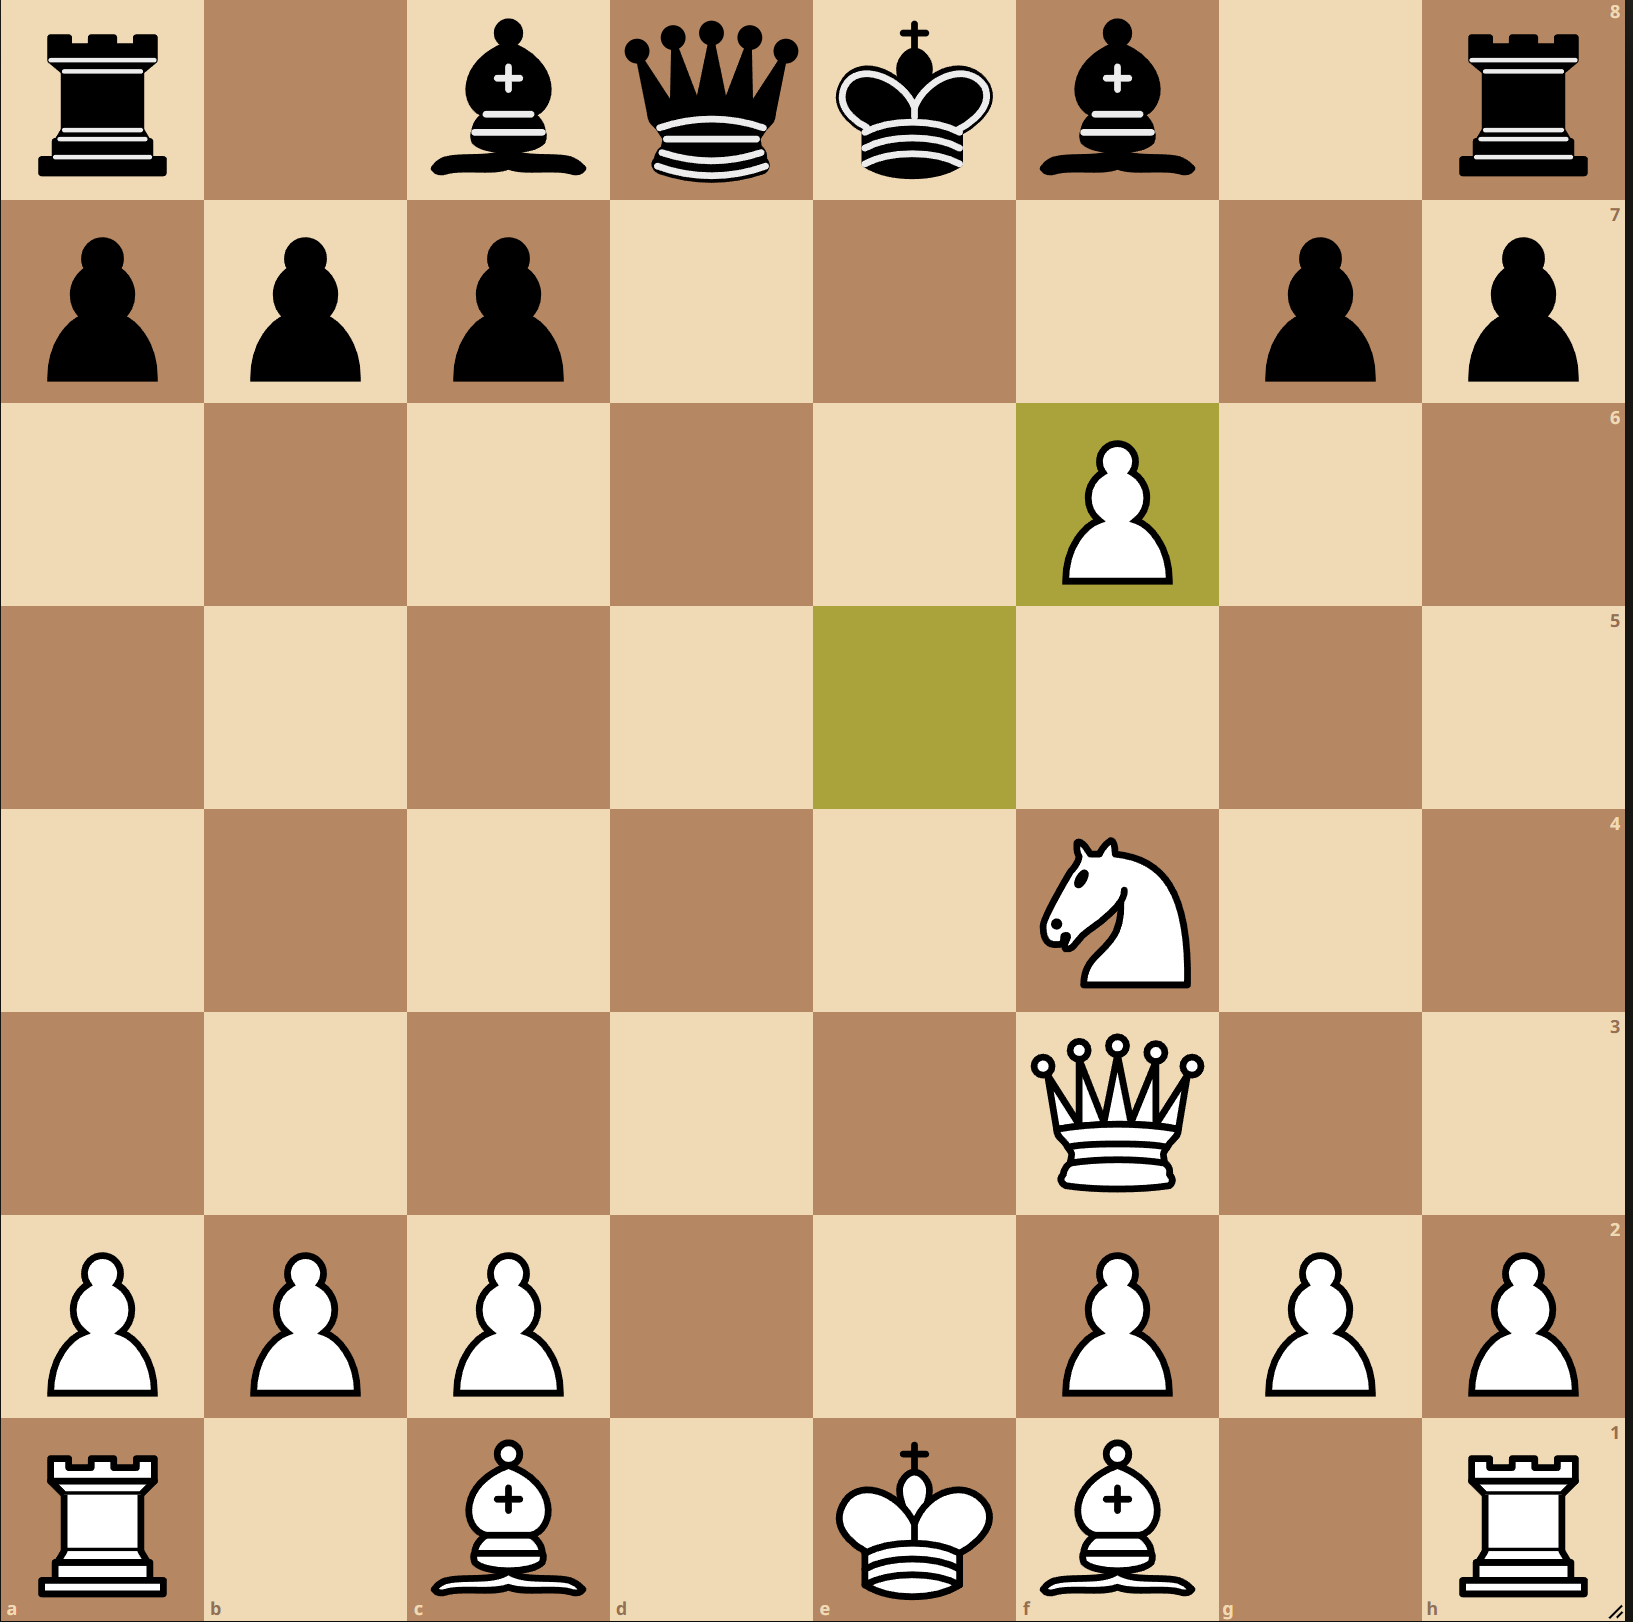
\includegraphics[width=\textwidth]{post_enpas.png}
        \caption{posizione della figura \ref{pre_enpas} post cattura con en passant}
    \end{minipage}
\end{figure}
Da un attenta lettura delle regole possiamo notare che la presa en passant sarà possibile in al massimo una casella per volta,
questo significa che, per indicare la presenza di un possibile presa è sufficiente utilizzare un intero, che avrà il valore della casella dove è
possibile catturare con en passant,trattandosi di un elemento della partita strettamente legato alle mosse, l'aspetto implementativo e di gestione verrà approfondito nella sottosezione \ref{move generation} dedicata alla generazione delle mosse


\section{Undo}
\label{undo}
\begin{figure}[H]
    \centering
    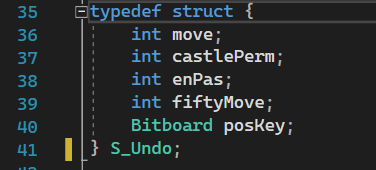
\includegraphics[width=\linewidth/2]{Undo.png}
\end{figure}
Struttura dati che contiene ogni mossa effettuata e lo stato della scacchiera prima che quella mossa venisse fatta,fondamentale per potere effettuare
il rollback della scacchiera ad uno stato precedente:
\begin{itemize}
    \item   \textbf{move}:
    \item   \textbf{castlePerm}:
    \item   \textbf{enPas}:
    \item   \textbf{fiftyMove}:
    \item   \textbf{poskey}:
\end{itemize}
